\section{Vooronderzoek}

\subsection{Neuraal netwerk}
Neurale netwerken zijn een reeks algoritmen die losjes gemodelleerd zijn van het menselijke brein. Een kunstmatig brein dat gemaakt is uit een hele grote reeks kunstmatige neuronen.

\subsubsection{Perceptrons}
Een van de meest fundamenteele kunstmatig neuron types is een perceptron.\cite{Perceptron1} Perceptronen zijn een belangrijk onderdeel van een neuraal netwerk en kennis hierover is nodig om een neuraal netwerk te begrijpen. Een perceptron pakt verschillende binary inputs:$x_{1}, x_{2},....x_{n}$ en produceerd een enkele binaire output. Je kan het zien als een functie die beslissingen voor je neemt, door verschillende factoren tegen elkaar te wegen en uiteindelijk met ja of nee te antwoorden.
\begin{figure}[h!]
\centering
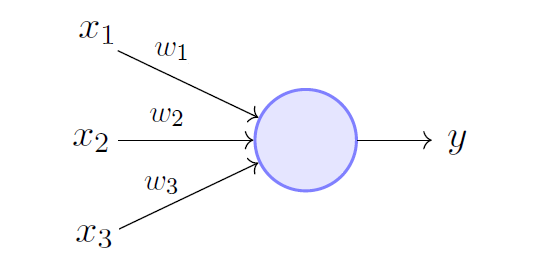
\includegraphics[scale=0.5]{perceptron2.png}
\caption{een enkelen perceptron}
\label{peceptron2}
\end{figure}
\linebreak
In afbeelding \ref{peceptron2} is een perceptron te zien die 3 variabelen als input neemt: $x_{1}, x_{2}$ en $x_{3}.$ Bij all deze waardes word een gewicht(weight) toegekend($w_{n}$). Deze waarde geeft aan hoe belangrijk de input is voor deze neuron. De output van de neuron is de som van alle resultaten bij elkaar. $\sum_{j}w_{j}x_{j}$ en deze waarde vergelijken met een gekozen randwaarde(threshold) om de output the berekenen. In een meer wiskundige term (w = weight, x = input en b = bias):

\begin{equation*}
\text{output perceptron}= \begin{cases}
0 &\text{if $\sum_{j}w_{j}x_{j}+ b \leq $ threshold }\\
1 &\text{if $\sum_{j}w_{j}x_{j}+ b>$ threshold }
\end{cases} 
\label{perceptron functie}
\end{equation*}
\newline
\noindent Je kan de output van een neuron beinvloeden door te spelen met de weights en thresholds. Door een input zijn weight te vergroten of de threshold te verlagen kan er hele andere resultaten uit het model komen\cite{NeuralNetwork1}. 
\newpage
\noindent Het is duidelijk dat de perceptron niet een compleet model is over hoe mensen hun beslissingen nemen. Maar het voorbeeld illustreert hoe een perceptron verschillende soorten bewijs kan afwegen om beslissingen te nemen. Daarom is het aannemelijk dat een complex netwerk van perceptrons vrij subtiele beslissingen zou moeten kunnen nemen\cite{NeuralNetwork1}.
\begin{figure}[h!]
\centering
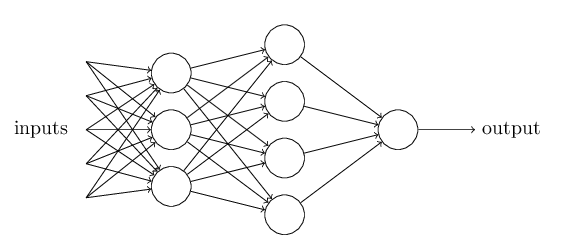
\includegraphics[scale=0.5]{perceptron3.png}
\caption{een neural network van meerderen perceptrons}
\label{perceptron3}
\end{figure}
\newline
In afbeelding \ref{perceptron3} is een netwerk te zien, waar de eerste laag van perceptrons in het netwerk, drie simpele beslissingen neemt door de functie in vergelijking \ref{perceptron fucntion} uit te voeren. Naast de eerste laag zit er nu ook een tweede die de outputs van de eerste laag als input neemt. Op deze manier kan een perceptron in de tweede laag een beslissing nemen op een complexer en abstracter niveau dan perceptrons in de eerste laag. Deze complexiteit en abstractheid word verhoogd per extra laag dat je toevoegd. Op deze manier kan een meerlaags netwerk van perceptrons, zeer geavanceerde beslissingen nemen\cite{NeuralNetwork1}\cite{learning}.\\ 
\newline
De volgende stap is om ons netwerk zelf lerend te maken. Om dit te doen moet je kleine aanpassingen kunnen maken aand de weights en de biases. Deze kleine aanpassingen moet daarna ook een klein effect hebben op de output van het neurale netwerk. Echter dat is niet wat er gebeurt met perceptronen want deze heeft maar 2 outputs, een 1 en een 0. Een kleine aanpassing zal daarom niks doen of de hele uitkomst van de perceptron omdraaien. Je kan niet probleem omzeilen door een ander types neurons te gebruiken ,zoals de Sigmoid en tanh neurons.\cite{learning}
\pagebreak
\subsubsection{Activatie functies}
De resultaten van een neuron worden berekend door een activatie functioes. Voor dit onderzoek worden eerst alleen de "Sigmoid" en "Tanh" activatie functies gebruikt, mochten deze niet goed werken worden andere activatie functies verder onderzocht\cite{learning}. \\\\
De sigmoid en tanh neurons lijken erg op perceptrons, alleen de manier hoe de ouput berekend wordt is compleet anders. Een sigmoid function neemt alle mogelijke nummers als een input en berekent het naar een getal tussen de 0 en 1.\\\\
\begin{equation}
    i_ \theta (x) =  \frac{\mathrm{1} }{\mathrm{1} + e^{-x} }  \label{sigmoid}
  \end{equation}
Een tanh functie neemt alle mogelijke nummers als input en brekend het naar en getal tussen de -1 en de 0.\\
\begin{equation}
    j_ \theta (x) =  \frac{\mathrm{2} }{\mathrm{1} + e^{-2x} } -1 \label{tanh}
  \end{equation}
  \linebreak
  \noindent De twee berekeningen lijken erg op elkaar, omdat tanh een geschaalde vorm is van de sigmoid functions.

\subsubsection{Zelf lerend netwerk}
Er is data nodig om een neuraal netwerk te trainen. Nadat deze data verzameld is kan er gebruik gemaakt worden van een methode die het neurale netwerk traint. Voorbeeld van zulke methodes zijn forward propagation, back propagation en resilent propagation. Het doel van deze algoritmes is om alle neuronen een weight en een bias te geven. Hoe dat in praktijk gaat hangt af van de dataset en welk algoritmn er gebruikt gaat worden, kort samengevat gaat het op deze manier\cite{learning}:
\begin{itemize}
\item De start waarden voor de weights en biases zijn vaak random.
\item De dataset wordt meegegeven aan het network en daar wordt data/resultaten uit gegenereerd.
\item Deze resultaten worden vergeleken met de verwachting en het foutpercentage/error wordt berekend.
\item Deze informatie wordt gebruikt om het het netwerk te tunen, zodat de error verminderd wordt.
\item De stappen worden herhaald tot het netwerk aan de eisen voldoet.
\end{itemize}

\subsubsection{Overfitting}
Neurale netwerken zijn erg kwetsbaar voor overfitting. Dit is als een neural netwerk alleen kan omgaan met de data uit een specifieke dataset en niet goed reageert op toekomstige waarnemingen\cite{algoritms}.\\ 
\newline
Overfiting onstaat door teveel factoren in het neurale netwerk op te nemen. Dit kan door heel veel specifieke data te geven aan het netwerk of door heel veel neuron te gebruiken die connecties gaan maken met die data. Als je deze dingen doet zal het netwerk altijd beter passend worden voor de gegevens die we al hebben, maar een betere pasvorm voor de beschikbare data betekent niet een betere prestatie\cite{algoritms}. \\
\newline
Dit klopt ook voor een netwerk met teweinig train data en/of neurons, als je er een te eenvoudig neural netwerk van maakt dan kan je het essentiele patroon in de data niet vastleggen. Een neural netwerk dat te gecompliceerd is word tegevoelig voor de specifiece data die we hadden vastgelegt. Als gevolg precies omdat het zo fijn is afgestemd op die specifieke train data gegeven word zal die voor oplossingen die met nieuwe informatie komen dan waar die me getrained is zwaar varieren en onbetrouwbare outputs geven\cite{algoritms}.\\
\newline
Dit is niet echt te verkomen, alleen door goed na tedenken over welke informatie je het netwerk zal laten geven, hoelang je het zal trainen en hoeveel neurons en layers het netwerk zal krijgen kan je zorgen dat je geen last krijgt van overfitting. De netwerken moet altijd getest worden of ze deze in de buurt komen van de resultaten die verwacht worden of dat ze inplaats daar van zijn getrained op test.\cite{algoritms}.
